%!TEX root = ../memoria.tex

\chapter{Formatos UTFSM para Memorias y Tesis de Grado }

Los formatos exigidos (y ocupados en este documento) por el Departamento de Industrias y la UTFSM incluyen:

\begin{description}
\item[Tipografía.] Fuente \emph{Times New Roman} o similar de 11 o 12 puntos (pts.), con interlineado de 1 espacio (máximo 1,5 espacios).
\item[Márgenes.] Margen izquierdo (o interno) de $3.5cm$ (mínimo). Margen derecho (o externo) de $2cm$ (mínimo). Note que esto cambia para páginas pares e impares para facilitar el empaste de documentos impresos por ambos lados de cada hoja.
\item[Citas bibliogáficas.] Las citas bibliográficas se harán siguiendo normas de la UTFSM (éstas están basadas en las normas \emph{APA} (usada en este documento), \emph{AMS}, o \emph{IEEE}). Ejemplo:

\begin{quote}
    ``\LaTeX{} es un sistema de diagramación de documentos.'' \citep{Lamport94}.
\end{quote}

Este documento ocupa estas normas. Revisar la bibliografía que se adjunta para ver un ejemplo.

\item[Numeración de Títulos.] El texto del informe final debe ser subdivido en: capítulos y sub-capítulos. La numeración de capítulos estará basada en esquema con división de puntos para los sub-capítulos, es decir: Capítulo 1, Sub-capítulo 1.1, etc.
\item[Numeración de Páginas.] Todas las páginas (con excepción de la portada) deben estar numeradas. El preámbulo (Índices, Resumen, Abstract, etc.) debe llevar numeración distinta del desarrollo (capítulos) del documento.
\item[Numeración de Formulas, Tablas y Figuras.] Las fórmulas, figuras y tablas correspondientes a un mismo capítulo, se identificarán mediante dos números. El primero corresponde al capítulo pertinente y el segundo al número de orden correlativo.


Los números con que se identifican las fórmulas se colocarán al extremo derecho de las mismas y entre paréntesis. Ejemplo (\autoref{eq:eq_example}):
\begin{equation}
f(x) = x^2-2x+1
\label{eq:eq_example}
\end{equation}

Las ilustraciones (gráficos, láminas, fotografías, etc.) en lo posible deben quedar ubicadas dentro de la página que se les referencia. Los números correspondientes a figuras se colocarán en la parte inferior de las mismas, seguidos de título o breve explicación de la figura. Ver \autoref{fig:figure_example}.
	\begin{figure}[ht!]
	\centering
	%\rule{4cm}{3cm}
	
\includegraphics[width=.3\textwidth]{figures/logoind.png}
	
	\caption[Logotipo del Departamento de Industrias, UTFSM.]{Logotipo del Departamento de Industrias, UTFSM.\\
	{\footnotesize (Fuente: Departamento de Industrias, 2016.)}}
	
	\label{fig:figure_example}
	\end{figure}

Los números asignados a las tablas se colocarán en la parte superior de ellas, seguidos de los títulos correspondientes. Ver \autoref{tbl:table_example}

\begin{table}[ht]
    \centering
    \caption[Ejemplo: Numeración de Tablas]{Ejemplo de Numeración de Tablas.}
    \begin{tabular}{@{}p{3cm}|p{3cm}|p{3cm}@{}}
        \toprule
        \textbf{Columna 1} & \textbf{Columna 2} & \textbf{Columna 3} \\
        \hline\hline
        ... & ... & ... \\
        \hline
        ... & ... & ... \\
        \hline
        ... & ... & ... \\
        \bottomrule
    \end{tabular}
    \label{tbl:table_example}
\end{table}

\end{description}

\section{Otros Formatos UTFSM}
\subsection{Formato de las Cubiertas (Empaste)}

A partir del año 2016, ya no es necesaria la entrega de una copia física de la memoria o tesis, siendo esto opcional. Si decide imprimirla, estás son las normas para el empaste.

La cubierta o tapa será de empaste duro, cubierta de vinilo o similar de color NEGRO con letras doradas, según se muestran en \autoref{fig:thesis_cover} y \autoref{fig:thesis_cover_lateral}.

\begin{figure}[ht!]
\centering
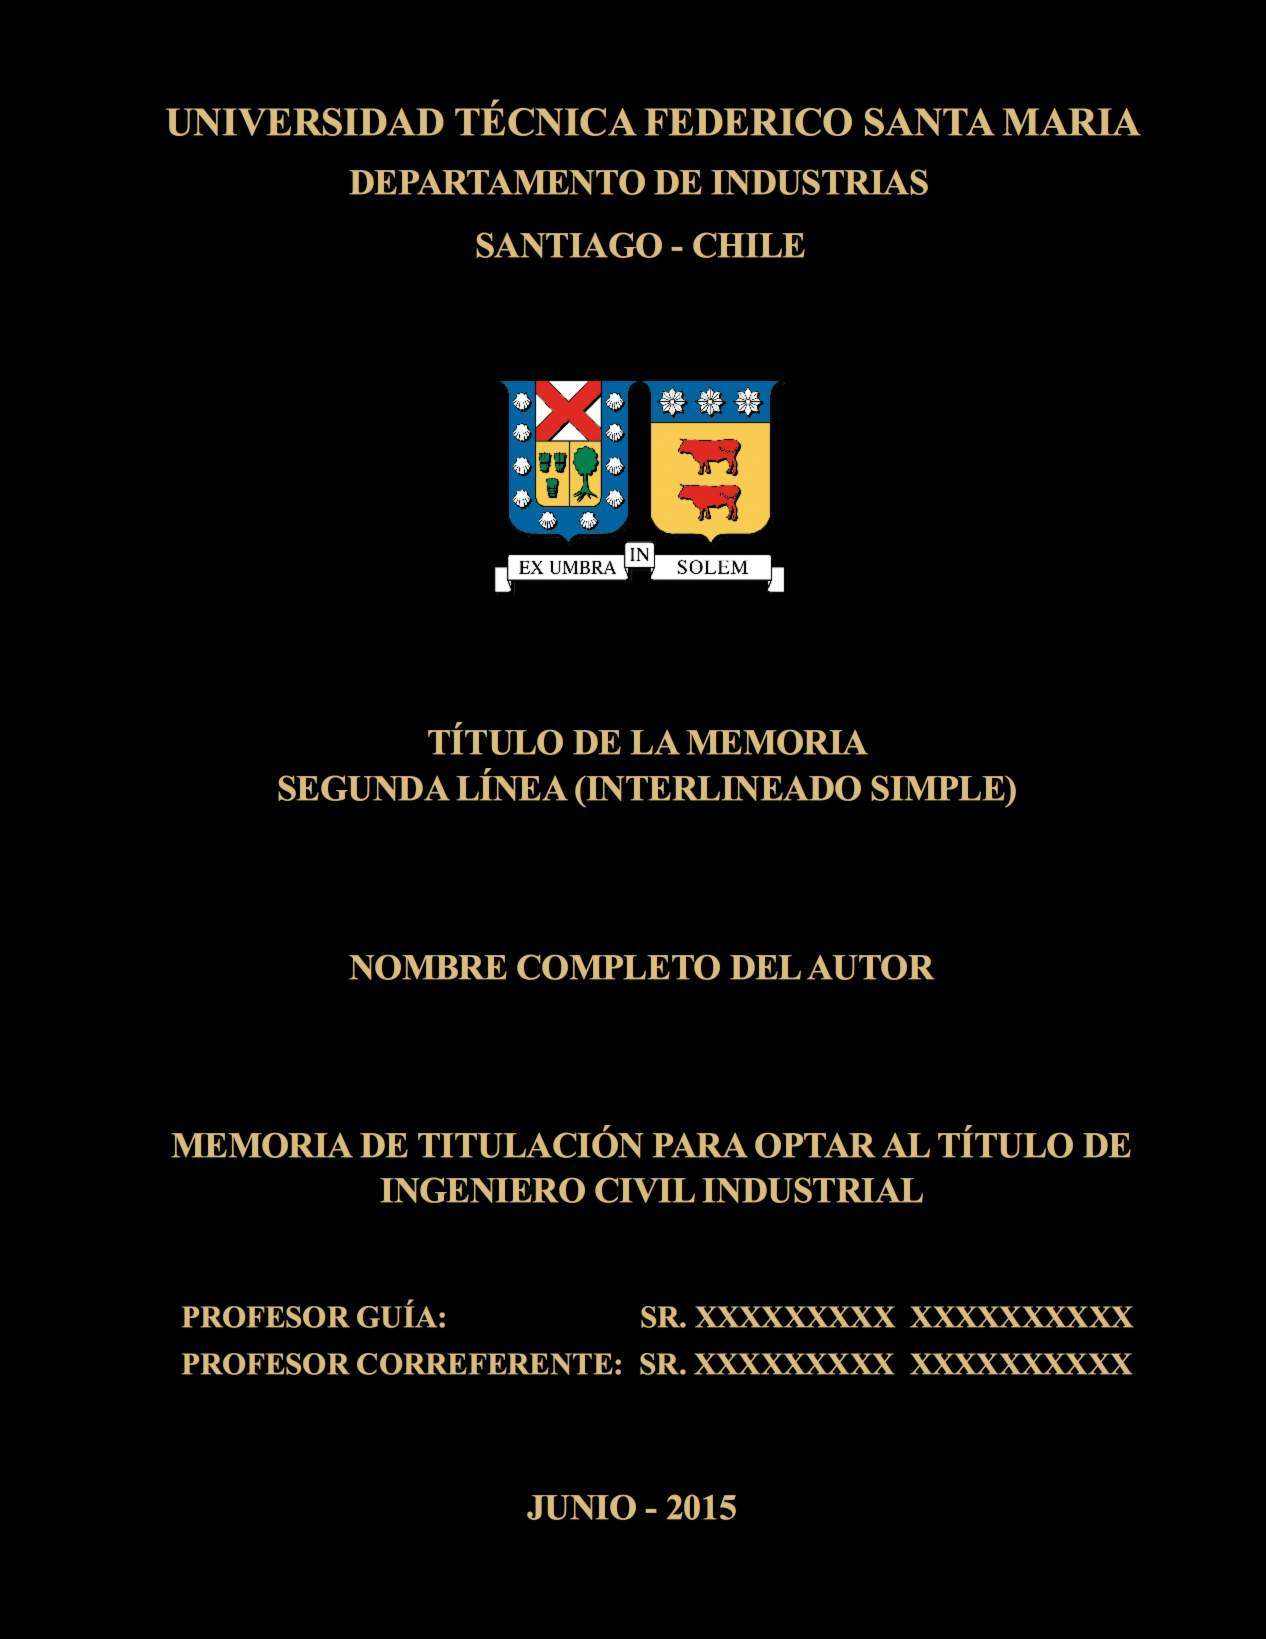
\includegraphics[width=.7\textwidth]{figures/thesis_cover.png}
\caption{Cubierta (Empaste) Memorias y Tesis UTFSM.}
\label{fig:thesis_cover}
\end{figure}

\begin{figure}[ht!]
\centering
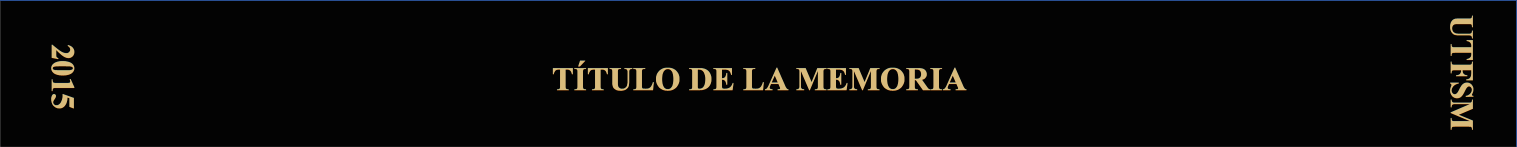
\includegraphics[width=.7\textwidth]{figures/thesis_cover_lateral.png}
\caption{Lomo del Empaste para Memorias y Tesis UTFSM.}
\label{fig:thesis_cover_lateral}
\end{figure}

\subsection{Formato del Disco Compacto}

El CD/DVD debe tener una carátula de identificación circular con fondo blanco, conteniendo las siguientes leyendas:

\begin{itemize}
		\item
    Centrado en la parte superior: UTFSM, con letras mayúsculas en negrita tamaño 12. A renglón seguido el nombre de la Unidad Académica con letras mayúsculas en negrita tamaño 10.
		\item
    Centrado en la parte inferior el nombre completo del alumno con letras mayúsculas en negrita tamaño 10.
		\item
    Tres espacios más abajo y centrado, “TÍTULO DE LA MEMORIA”, con letras mayúsculas en negrita tamaño 10.
		\item
    Dos espacios más abajo y centrado MES –AÑO, con letras mayúsculas en negrita tamaño 10.
    En el lado izquierdo y centrado, el escudo en colores de la Institución.
		\item
    En el lado derecho y centrado, NOMBRE DE LA UNIDAD ACADÉMICA y la ubicación CIUDAD – PAIS, con letras mayúsculas en negrita tamaño 8.
\end{itemize}

\begin{figure}[ht!]
\centering
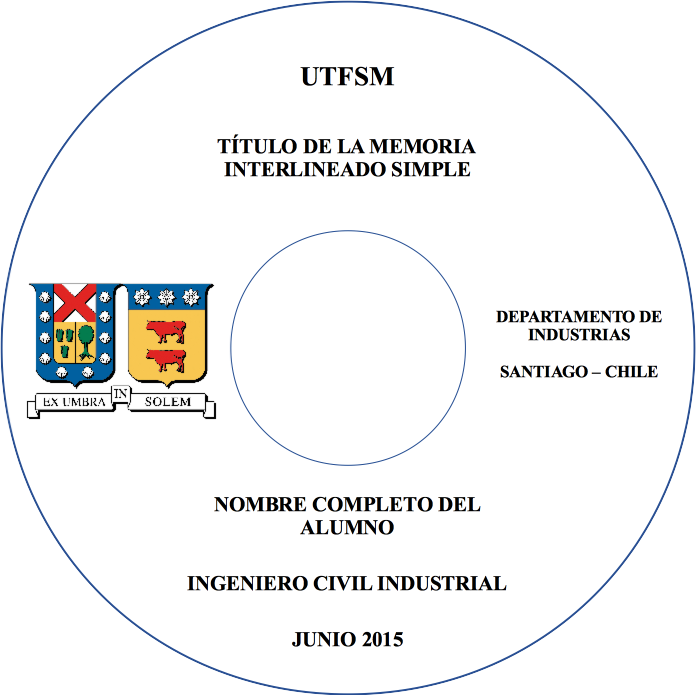
\includegraphics[width=.4\textwidth]{figures/thesis_cd.png}
\caption{Disco Compacto para Memoria UTFSM}
\label{fig:thesis_cd}
\end{figure}


Los CD se guardarán, en la biblioteca, en una caja de acrílico que tendrá una carátula de identificación dividida en tres franjas iguales, con las siguientes leyendas:
\begin{itemize}
		\item
    El escudo a color de la Institución de 20 mm de alto, centrado en la franja superior.
		\item
    El nombre completo del alumno, y centrado dos espacios más abajo el título de la memoria, en la franja del medio
		\item
    El nombre de la Unidad Académica, y renglón más abajo, año. En la franja inferior.
\end{itemize}


\begin{figure}[ht!]
    \centering
    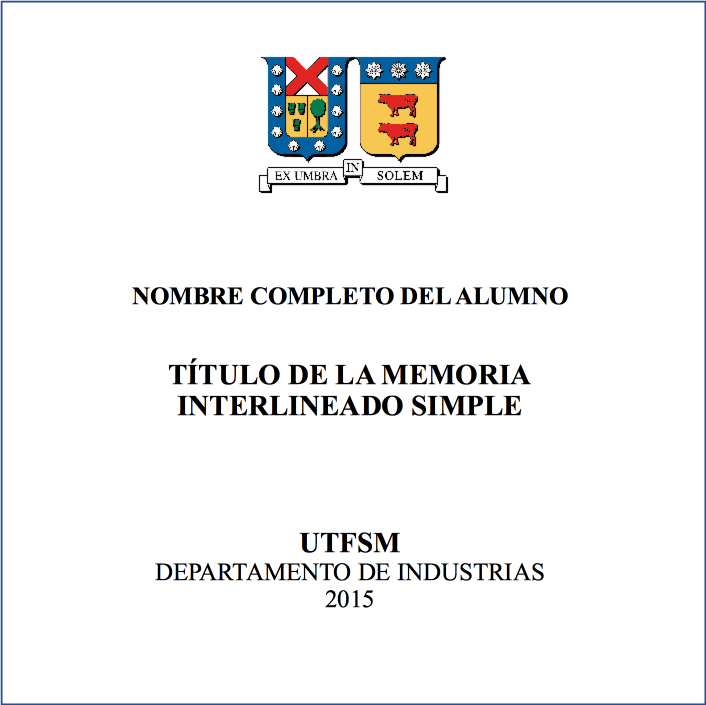
\includegraphics[width=.4\textwidth]{figures/thesis_cd_cover.png}
    \caption{Cubierta de Disco Compacto para Memorias y Tesis UTFSM.}
    \label{fig:thesis_cd_cover}
\end{figure}


La carpeta \inlinecode{figures} incluye los diagramas (formato LibreOffice) para modificación e impresión.

%%%%%
\section{Documentos que se incluyen}

Se incluyen (en la carpeta \inlinecode{figures}) logotipos oficiales\footnote{Éstas son imágenes registradas y propiedad intelectual de la UTFSM y del Departamento de Industrias, y no están incluidas en la licencia de esta plantilla. La imagen corporativa de la UTFSM y del Departamento de Industrias están protegidas por leyes chilenas e internacionales de Derechos de autor. Su uso sólo está autorizado a estudiantes y memoristas de la UTFSM para fines de preparación de documentos académicos, incluidas memorias y tesis.}
de la UTFSM y del Departamento de Industrias.

\begin{figure}[ht!]
\centering

\includegraphics[scale = .5]{figures/logousm.png}
\caption{Logotipo de la UTFSM}
\label{fig:logousm}
\end{figure}

\begin{figure}[ht!]
\centering

\includegraphics[scale = .45]{figures/logousmleyenda.png}
\caption{Logotipo de la UTFSM (con leyenda)}
\label{fig:logousmleyenda}
\end{figure}


\begin{figure}[ht!]
\centering

\includegraphics[scale = .75]{figures/logousmind.jpg}
\caption{Logotipo de la UTFSM - Departamento de Industrias}
\label{fig:logousmind}
\end{figure}

\begin{figure}[ht!]
    \centering
    %\rule{4cm}{3cm}
    
\includegraphics[width=.8\textwidth]{figures/logo_utfsm_di.png}
    \caption{Logotipo del Departamento de Industrias, UTFSM (Formato lateral).}
    \label{fig:logodiutfsm}
\end{figure}

\begin{figure}[ht!]
\centering
%\rule{4cm}{3cm}

\includegraphics[width=.3\textwidth]{figures/logoind.png}
\caption{Logotipo del Departamento de Industrias, UTFSM }
\label{fig:logoind1}
\end{figure}

